\section[Реализация программного модуля]{%
  РЕАЛИЗАЦИЯ ПРОГРАММНОГО МОДУЛЯ
}\label{sec:implementation}

Данный раздел содержит подробное описание деталей реализации
мобильного приложения, дополняя и уточняя
содержание раздела~\ref{sec:design}.

\subsection{Выбор программных средств реализации}

Мобильная платформа Android в значительной мере
определяет набор средств разработки. Большинство Android-приложений
разрабатываются на языке программирования Java. Программирование
приложения производится c помощью специализированной
IDE Android Studio с использованием Android Software Developement Kit (SDK).

Существует некоторая свобода выбора в отношении используемой СУБД.
Следует отметить, что системы управления базами данных,
используемые на мобильных платформах, существенно отличаются
от традиционных решений.
Это вызвано тем, что работа мобильных баз данных производится в
иных условиях, характеризующися следующими особенностями:
\begin{itemize}
  \item малый рабочий объем данных;
  \item низкая плотность потока запросов обработки данных;
  \item отсутствие необходимости обработки параллельных транзакций;
  \item программный интерфейс приложения-клиента заранее известен.
\end{itemize}

Первые три условия вызваны тем, что СУБД обрабатывает запросы
лишь одного клиента --- пользователя приложения.
Последнее условие вызвано тем, что программный интерфейс мобильных
приложений для платформы Android известен по определению (Java VM).

С другой стороны, мобильные платформы выдвигают ряд
дополнительных требований к СУБД.
Во-первых, работа базы данных должна производиться в рамках
процесса клиентского приложения, поскольку Android не гаратирует
неприкосновенности пользовательских процессов, то есть они могут быть
приостановлены или завершены в любой момент времени.
Во-вторых, механизм хранения данных должен быть централизованным,
компактным и переносимым. Это требование накладывает
известные ограничения на используемые структуры данных
и алгоритмы их обработки.

Существует несколько популярных СУБД для мобильных устройств.
По умолчанию Android предоставляет возможность хранения
данных с использованием SQLite --- малой реляционной СУБД,
используемой также и на персональных компьютерах.
Характерными особенностями данной СУБД являются поддержка SQL,
хранение данных в едином файле и отсутствие необходимости конфигурирования.
Кроме этого, существует несколько альтернативных СУБД~\cite{mobile_db}:
Cupboard, BerkeleyDB, Couchbase Lite, LevelDB, Realm, UnQLite.

В разрабатываемом приложении используется СУБД Realm~\cite{realm_official}.
Выбор обусловлен следующими причинами:
\begin{itemize}
  \item Realm является объектно-ориентированной СУБД,
    что избавляет от необходимости написания слоя трансляции объектов Java
    в сущности реляционной БД (ORM);
  \item Realm имеет более высокую производительность, чем решения на базе SQLite;
  \item проект активно развивается, является открытым,
    бесплатным для коммерческого использования,
    а также имеет подробную документацию.
\end{itemize}

Кроме этого, разрабатываемое приложение использует библиотеку OpenCV
для обработки и распознавания изображений, а также библиотеки Appcompat
(реализация рекомендаций Material Design на старых версиях платформы Android)
и JUnit (для тестирования приложения).

\subsection{Реализация подсистемы хранения данных}
\label{subsec:implementation_db}

Поскольку Realm является объектно-ориентированной СУБД,
сущности модели данных, разработанной в подразделе~\ref{subsec:design_information},
находят свое прямое отражение в классах Java.
При этом Realm предъявляет следующие дополнительные требования
к классам модели данных:
\begin{itemize}
  \item данные классы должны быть унаследованы от \texttt{RealmObject};
  \item каждый класс иметь публичный конструктор без параметров,
    а также набор соответствующих методов доступа/модификации полей данных;
  \item набор типов хранимых данных ограничен набором базовых типов,
    а также другими классами модели данных.
\end{itemize}

Realm поддерживает хранение следующих базовых типов данных:
\texttt{boolean}, \texttt{byte}, \texttt{short}, \texttt{ìnt},
\texttt{long}, \texttt{float}, \texttt{double}, \texttt{String},
\texttt{Date} и \texttt{byte[]}.
Кроме этого, поддерживается возможность создания отношений вида
1:1, 1:M, M:M путем хранения наборов ссылок на другие объекты Realm
в виде списков (\texttt{RealmList}).

На рисунке~\ref{lst:implementation_db_account} представлен класс
\texttt{Account}, соответствующий сущности <<УчетнаяЗапись>> исходной
модели данных.
Данный класс является публичным, унаследованным от класса \texttt{RealmObject}.
Он содержит набор приватных полей данных: название, индекс, код валюты,
а также список связанных объектов \texttt{BalanceChange},
соответствующих изменениям баланса.
Кроме этого, он содержит публичное строковое поле, соответствующее
названию поля индекса и используемое для сортировки.

\lstinputlisting[
    caption=Пример класса модели данных,
    language={Java},
    label=lst:implementation_db_account,
]{lst/implementation_db_account.lst}

Большинство методов класса выполняют чтение/модификацию
полей объекта; метод \texttt{getBalanceChanges} возвращает ссылку на
список связанных изменений баланса,
а метод \texttt{getTotalAmount} использует встроенную
агрегатную функцию для получения суммы значений данных изменений.

Доступ к подсистеме базы данных осуществляется через класс
\texttt{DBManager}. Данный класс представляет собой синглтон,
выполняющий инициализацию и контроль доступа к объектам \texttt{Realm}
стороны подсистемы обработки данных.

Полный исходный код реализации модели данных представлен в приложении~А.

\subsection{Реализация подсистемы компьютерного зрения}
\label{subsec:implementation_cv}

Подсистема компьютерного зрения реализована на базе библиотеки
OpenCV и носит экспериментальный характер.

\subsection{Реализация пользовательского интерфейса}
\label{subsec:implementation_ui}

Данный подраздел рассматривает детали реализации пользовательского
интерфейса приложения.
Вначале рассматриваются принципы организации программного
графического интерфейса платформы Android в целом,
далее описывается подход к обработке и отображению пользовательских данных,
затем приводится подробное описание элементов интерфейса различных
экранов приложения, введенных в подразделе~\ref{subsec:design_structure}.

Графический интерфейс платформы Android базируется на трех классах:
\texttt{Activity}, \texttt{Fragment} и \texttt{View}.
Класс \texttt{Activity} (экран) соответствует отдельному экрану приложения.
Класс \texttt{Fragment} (фрагмент) соответствует относительно самостоятельной части
экрана приложения.
Экраны и фрагменты содержат множество экземпляров класса \texttt{View},
соответствующего базовым элементам интерфейса --- полям, кнопкам, и~т.~д.
Взаимосвязь этих классов приведена на рисунке~\ref{fig:implementation_ui_hierarchy}.

\begin{figure}[h!]
  \centering
  \fcolorbox{gray}{white}{
    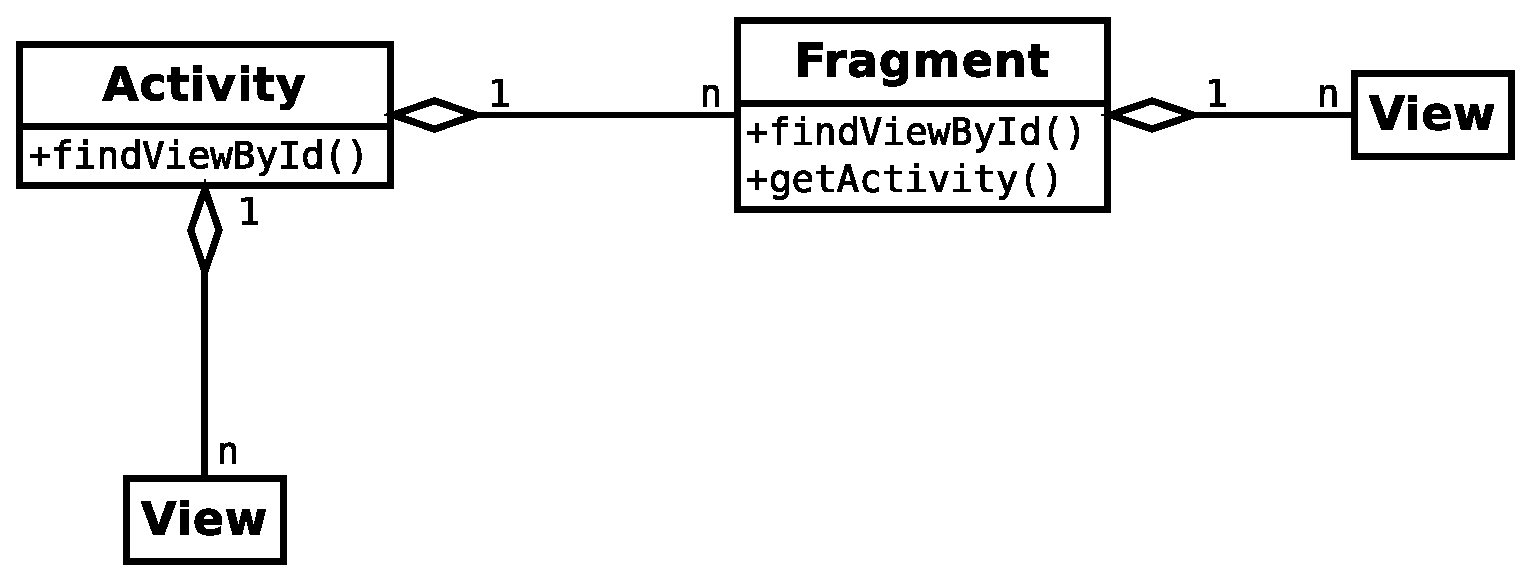
\includegraphics[width=140mm]{fig/implementation_ui_hierarchy.eps}
  }
  \caption{Организация базовых классов \\ пользовательского интерфейса Android}
  \label{fig:implementation_ui_hierarchy}
\end{figure}

Введение понятия фрагмента обусловлено необходимостью унификации
механизма поддержки пользовательского интерфейса для устройств с различным
размером дисплея. Так, например, на устройствах с большим размером дисплея
один экран приложения может содержать несколько фрагментов, а на малом ---
каждый фрагмент будет находиться в отдельном экране.
Связь между экраном и фрагментом осуществляется явно:
экраны хранят ссылки на созданные ими фрагменты,
а фрагменты могут получить ссылку на родительские экраны путем
вызова метода \texttt{getActivity}.
Для получения ссылки на требуемый объект класса \texttt{View}
используется метод \texttt{findViewById}.

Платформа Android управляет экранами и фрагментами путем вызова ряда методов,
определенных в базовых классах. Совокупность данных методов образует
жизненный цикл элемента интерфейса. Каждый из них принимает
специльный аргумент типа \texttt{Bundle}, позволяющий передавать
аргументы примитивных типов, а также сохранять и восстанавливать
собственное состояние.
На рисунке~\ref{fig:implementation_ui_lifecycle_activity}
представлена схема жизненного цикла экрана приложения.

\begin{figure}[h!]
  \centering
  \fcolorbox{gray}{white}{% Graphic for TeX using PGF
% Title: /home/budnyjj/univer/GIT/diploma/b/design/diagrams/lifecycle_activity.dia
% Creator: Dia v0.97.3
% CreationDate: Tue May 10 10:33:42 2016
% For: budnyjj
% \usepackage{tikz}
% The following commands are not supported in PSTricks at present
% We define them conditionally, so when they are implemented,
% this pgf file will use them.
\ifx\du\undefined
  \newlength{\du}
\fi
\setlength{\du}{15\unitlength}
\begin{tikzpicture}
\pgftransformxscale{1.000000}
\pgftransformyscale{-1.000000}
\definecolor{dialinecolor}{rgb}{0.000000, 0.000000, 0.000000}
\pgfsetstrokecolor{dialinecolor}
\definecolor{dialinecolor}{rgb}{1.000000, 1.000000, 1.000000}
\pgfsetfillcolor{dialinecolor}
\pgfsetlinewidth{0.100000\du}
\pgfsetdash{}{0pt}
\pgfsetdash{}{0pt}
\pgfsetbuttcap
\pgfsetmiterjoin
\pgfsetlinewidth{0.100000\du}
\pgfsetbuttcap
\pgfsetmiterjoin
\pgfsetdash{}{0pt}
\definecolor{dialinecolor}{rgb}{1.000000, 1.000000, 1.000000}
\pgfsetfillcolor{dialinecolor}
\pgfpathmoveto{\pgfpoint{13.339950\du}{9.006000\du}}
\pgfpathlineto{\pgfpoint{17.127450\du}{9.006000\du}}
\pgfpathcurveto{\pgfpoint{17.650395\du}{9.006000\du}}{\pgfpoint{18.074325\du}{9.576090\du}}{\pgfpoint{18.074325\du}{10.279333\du}}
\pgfpathcurveto{\pgfpoint{18.074325\du}{10.982576\du}}{\pgfpoint{17.650395\du}{11.552667\du}}{\pgfpoint{17.127450\du}{11.552667\du}}
\pgfpathlineto{\pgfpoint{13.339950\du}{11.552667\du}}
\pgfpathcurveto{\pgfpoint{12.817005\du}{11.552667\du}}{\pgfpoint{12.393075\du}{10.982576\du}}{\pgfpoint{12.393075\du}{10.279333\du}}
\pgfpathcurveto{\pgfpoint{12.393075\du}{9.576090\du}}{\pgfpoint{12.817005\du}{9.006000\du}}{\pgfpoint{13.339950\du}{9.006000\du}}
\pgfusepath{fill}
\definecolor{dialinecolor}{rgb}{0.000000, 0.000000, 0.000000}
\pgfsetstrokecolor{dialinecolor}
\pgfpathmoveto{\pgfpoint{13.339950\du}{9.006000\du}}
\pgfpathlineto{\pgfpoint{17.127450\du}{9.006000\du}}
\pgfpathcurveto{\pgfpoint{17.650395\du}{9.006000\du}}{\pgfpoint{18.074325\du}{9.576090\du}}{\pgfpoint{18.074325\du}{10.279333\du}}
\pgfpathcurveto{\pgfpoint{18.074325\du}{10.982576\du}}{\pgfpoint{17.650395\du}{11.552667\du}}{\pgfpoint{17.127450\du}{11.552667\du}}
\pgfpathlineto{\pgfpoint{13.339950\du}{11.552667\du}}
\pgfpathcurveto{\pgfpoint{12.817005\du}{11.552667\du}}{\pgfpoint{12.393075\du}{10.982576\du}}{\pgfpoint{12.393075\du}{10.279333\du}}
\pgfpathcurveto{\pgfpoint{12.393075\du}{9.576090\du}}{\pgfpoint{12.817005\du}{9.006000\du}}{\pgfpoint{13.339950\du}{9.006000\du}}
\pgfusepath{stroke}
% setfont left to latex
\definecolor{dialinecolor}{rgb}{0.000000, 0.000000, 0.000000}
\pgfsetstrokecolor{dialinecolor}
\node at (15.233700\du,10.448667\du){Начало};
\definecolor{dialinecolor}{rgb}{1.000000, 1.000000, 1.000000}
\pgfsetfillcolor{dialinecolor}
\fill (12.936200\du,12.774600\du)--(12.936200\du,15.321267\du)--(17.531200\du,15.321267\du)--(17.531200\du,12.774600\du)--cycle;
\pgfsetlinewidth{0.100000\du}
\pgfsetdash{}{0pt}
\pgfsetdash{}{0pt}
\pgfsetmiterjoin
\definecolor{dialinecolor}{rgb}{0.000000, 0.000000, 0.000000}
\pgfsetstrokecolor{dialinecolor}
\draw (12.936200\du,12.774600\du)--(12.936200\du,15.321267\du)--(17.531200\du,15.321267\du)--(17.531200\du,12.774600\du)--cycle;
% setfont left to latex
\definecolor{dialinecolor}{rgb}{0.000000, 0.000000, 0.000000}
\pgfsetstrokecolor{dialinecolor}
\node at (15.233700\du,14.227100\du){onCreate()};
\definecolor{dialinecolor}{rgb}{1.000000, 1.000000, 1.000000}
\pgfsetfillcolor{dialinecolor}
\fill (13.179950\du,16.705430\du)--(13.179950\du,19.252097\du)--(17.287450\du,19.252097\du)--(17.287450\du,16.705430\du)--cycle;
\pgfsetlinewidth{0.100000\du}
\pgfsetdash{}{0pt}
\pgfsetdash{}{0pt}
\pgfsetmiterjoin
\definecolor{dialinecolor}{rgb}{0.000000, 0.000000, 0.000000}
\pgfsetstrokecolor{dialinecolor}
\draw (13.179950\du,16.705430\du)--(13.179950\du,19.252097\du)--(17.287450\du,19.252097\du)--(17.287450\du,16.705430\du)--cycle;
% setfont left to latex
\definecolor{dialinecolor}{rgb}{0.000000, 0.000000, 0.000000}
\pgfsetstrokecolor{dialinecolor}
\node at (15.233700\du,18.157930\du){onStart()};
\definecolor{dialinecolor}{rgb}{1.000000, 1.000000, 1.000000}
\pgfsetfillcolor{dialinecolor}
\fill (12.728700\du,20.610400\du)--(12.728700\du,23.157067\du)--(17.738700\du,23.157067\du)--(17.738700\du,20.610400\du)--cycle;
\pgfsetlinewidth{0.100000\du}
\pgfsetdash{}{0pt}
\pgfsetdash{}{0pt}
\pgfsetmiterjoin
\definecolor{dialinecolor}{rgb}{0.000000, 0.000000, 0.000000}
\pgfsetstrokecolor{dialinecolor}
\draw (12.728700\du,20.610400\du)--(12.728700\du,23.157067\du)--(17.738700\du,23.157067\du)--(17.738700\du,20.610400\du)--cycle;
% setfont left to latex
\definecolor{dialinecolor}{rgb}{0.000000, 0.000000, 0.000000}
\pgfsetstrokecolor{dialinecolor}
\node at (15.233700\du,22.062900\du){onResume()};
\definecolor{dialinecolor}{rgb}{1.000000, 1.000000, 1.000000}
\pgfsetfillcolor{dialinecolor}
\fill (13.028700\du,29.282600\du)--(13.028700\du,31.829267\du)--(17.438700\du,31.829267\du)--(17.438700\du,29.282600\du)--cycle;
\pgfsetlinewidth{0.100000\du}
\pgfsetdash{}{0pt}
\pgfsetdash{}{0pt}
\pgfsetmiterjoin
\definecolor{dialinecolor}{rgb}{0.000000, 0.000000, 0.000000}
\pgfsetstrokecolor{dialinecolor}
\draw (13.028700\du,29.282600\du)--(13.028700\du,31.829267\du)--(17.438700\du,31.829267\du)--(17.438700\du,29.282600\du)--cycle;
% setfont left to latex
\definecolor{dialinecolor}{rgb}{0.000000, 0.000000, 0.000000}
\pgfsetstrokecolor{dialinecolor}
\node at (15.233700\du,30.735100\du){onPause()};
\definecolor{dialinecolor}{rgb}{1.000000, 1.000000, 1.000000}
\pgfsetfillcolor{dialinecolor}
\fill (13.196200\du,33.229400\du)--(13.196200\du,35.776067\du)--(17.271200\du,35.776067\du)--(17.271200\du,33.229400\du)--cycle;
\pgfsetlinewidth{0.100000\du}
\pgfsetdash{}{0pt}
\pgfsetdash{}{0pt}
\pgfsetmiterjoin
\definecolor{dialinecolor}{rgb}{0.000000, 0.000000, 0.000000}
\pgfsetstrokecolor{dialinecolor}
\draw (13.196200\du,33.229400\du)--(13.196200\du,35.776067\du)--(17.271200\du,35.776067\du)--(17.271200\du,33.229400\du)--cycle;
% setfont left to latex
\definecolor{dialinecolor}{rgb}{0.000000, 0.000000, 0.000000}
\pgfsetstrokecolor{dialinecolor}
\node at (15.233700\du,34.681900\du){onStop()};
\definecolor{dialinecolor}{rgb}{1.000000, 1.000000, 1.000000}
\pgfsetfillcolor{dialinecolor}
\fill (12.747450\du,37.353000\du)--(12.747450\du,39.899667\du)--(17.719950\du,39.899667\du)--(17.719950\du,37.353000\du)--cycle;
\pgfsetlinewidth{0.100000\du}
\pgfsetdash{}{0pt}
\pgfsetdash{}{0pt}
\pgfsetmiterjoin
\definecolor{dialinecolor}{rgb}{0.000000, 0.000000, 0.000000}
\pgfsetstrokecolor{dialinecolor}
\draw (12.747450\du,37.353000\du)--(12.747450\du,39.899667\du)--(17.719950\du,39.899667\du)--(17.719950\du,37.353000\du)--cycle;
% setfont left to latex
\definecolor{dialinecolor}{rgb}{0.000000, 0.000000, 0.000000}
\pgfsetstrokecolor{dialinecolor}
\node at (15.233700\du,38.805500\du){onDestroy()};
\pgfsetlinewidth{0.100000\du}
\pgfsetdash{}{0pt}
\pgfsetdash{}{0pt}
\pgfsetbuttcap
\pgfsetmiterjoin
\pgfsetlinewidth{0.100000\du}
\pgfsetbuttcap
\pgfsetmiterjoin
\pgfsetdash{}{0pt}
\definecolor{dialinecolor}{rgb}{1.000000, 1.000000, 1.000000}
\pgfsetfillcolor{dialinecolor}
\pgfpathmoveto{\pgfpoint{13.489950\du}{41.429500\du}}
\pgfpathlineto{\pgfpoint{16.977450\du}{41.429500\du}}
\pgfpathcurveto{\pgfpoint{17.458973\du}{41.429500\du}}{\pgfpoint{17.849325\du}{41.999590\du}}{\pgfpoint{17.849325\du}{42.702833\du}}
\pgfpathcurveto{\pgfpoint{17.849325\du}{43.406076\du}}{\pgfpoint{17.458973\du}{43.976167\du}}{\pgfpoint{16.977450\du}{43.976167\du}}
\pgfpathlineto{\pgfpoint{13.489950\du}{43.976167\du}}
\pgfpathcurveto{\pgfpoint{13.008427\du}{43.976167\du}}{\pgfpoint{12.618075\du}{43.406076\du}}{\pgfpoint{12.618075\du}{42.702833\du}}
\pgfpathcurveto{\pgfpoint{12.618075\du}{41.999590\du}}{\pgfpoint{13.008427\du}{41.429500\du}}{\pgfpoint{13.489950\du}{41.429500\du}}
\pgfusepath{fill}
\definecolor{dialinecolor}{rgb}{0.000000, 0.000000, 0.000000}
\pgfsetstrokecolor{dialinecolor}
\pgfpathmoveto{\pgfpoint{13.489950\du}{41.429500\du}}
\pgfpathlineto{\pgfpoint{16.977450\du}{41.429500\du}}
\pgfpathcurveto{\pgfpoint{17.458973\du}{41.429500\du}}{\pgfpoint{17.849325\du}{41.999590\du}}{\pgfpoint{17.849325\du}{42.702833\du}}
\pgfpathcurveto{\pgfpoint{17.849325\du}{43.406076\du}}{\pgfpoint{17.458973\du}{43.976167\du}}{\pgfpoint{16.977450\du}{43.976167\du}}
\pgfpathlineto{\pgfpoint{13.489950\du}{43.976167\du}}
\pgfpathcurveto{\pgfpoint{13.008427\du}{43.976167\du}}{\pgfpoint{12.618075\du}{43.406076\du}}{\pgfpoint{12.618075\du}{42.702833\du}}
\pgfpathcurveto{\pgfpoint{12.618075\du}{41.999590\du}}{\pgfpoint{13.008427\du}{41.429500\du}}{\pgfpoint{13.489950\du}{41.429500\du}}
\pgfusepath{stroke}
% setfont left to latex
\definecolor{dialinecolor}{rgb}{0.000000, 0.000000, 0.000000}
\pgfsetstrokecolor{dialinecolor}
\node at (15.233700\du,42.872167\du){Конец};
\pgfsetlinewidth{0.100000\du}
\pgfsetdash{}{0pt}
{\pgfsetcornersarced{\pgfpoint{0.500000\du}{0.500000\du}}\definecolor{dialinecolor}{rgb}{1.000000, 1.000000, 1.000000}
\pgfsetfillcolor{dialinecolor}
\fill (11.166200\du,24.525500\du)--(11.166200\du,27.783278\du)--(19.301200\du,27.783278\du)--(19.301200\du,24.525500\du)--cycle;
}{\pgfsetcornersarced{\pgfpoint{0.500000\du}{0.500000\du}}\definecolor{dialinecolor}{rgb}{0.000000, 0.000000, 0.000000}
\pgfsetstrokecolor{dialinecolor}
\draw (11.166200\du,24.525500\du)--(11.166200\du,27.783278\du)--(19.301200\du,27.783278\du)--(19.301200\du,24.525500\du)--cycle;
}% setfont left to latex
\definecolor{dialinecolor}{rgb}{0.000000, 0.000000, 0.000000}
\pgfsetstrokecolor{dialinecolor}
\node at (15.233700\du,25.830500\du){Взаимодействие с };
% setfont left to latex
\definecolor{dialinecolor}{rgb}{0.000000, 0.000000, 0.000000}
\pgfsetstrokecolor{dialinecolor}
\node at (15.233700\du,26.959389\du){пользователем};
\definecolor{dialinecolor}{rgb}{1.000000, 1.000000, 1.000000}
\pgfsetfillcolor{dialinecolor}
\fill (19.654514\du,16.705430\du)--(19.654514\du,19.252097\du)--(24.399514\du,19.252097\du)--(24.399514\du,16.705430\du)--cycle;
\pgfsetlinewidth{0.100000\du}
\pgfsetdash{}{0pt}
\pgfsetdash{}{0pt}
\pgfsetmiterjoin
\definecolor{dialinecolor}{rgb}{0.000000, 0.000000, 0.000000}
\pgfsetstrokecolor{dialinecolor}
\draw (19.654514\du,16.705430\du)--(19.654514\du,19.252097\du)--(24.399514\du,19.252097\du)--(24.399514\du,16.705430\du)--cycle;
% setfont left to latex
\definecolor{dialinecolor}{rgb}{0.000000, 0.000000, 0.000000}
\pgfsetstrokecolor{dialinecolor}
\node at (22.027014\du,18.157930\du){onRestart()};
\pgfsetlinewidth{0.100000\du}
\pgfsetdash{}{0pt}
\pgfsetdash{}{0pt}
\pgfsetbuttcap
{
\definecolor{dialinecolor}{rgb}{0.000000, 0.000000, 0.000000}
\pgfsetfillcolor{dialinecolor}
% was here!!!
\pgfsetarrowsend{to}
\definecolor{dialinecolor}{rgb}{0.000000, 0.000000, 0.000000}
\pgfsetstrokecolor{dialinecolor}
\draw (15.233700\du,11.602852\du)--(15.233700\du,12.724415\du);
}
\pgfsetlinewidth{0.100000\du}
\pgfsetdash{}{0pt}
\pgfsetdash{}{0pt}
\pgfsetbuttcap
{
\definecolor{dialinecolor}{rgb}{0.000000, 0.000000, 0.000000}
\pgfsetfillcolor{dialinecolor}
% was here!!!
\pgfsetarrowsend{to}
\definecolor{dialinecolor}{rgb}{0.000000, 0.000000, 0.000000}
\pgfsetstrokecolor{dialinecolor}
\draw (15.233700\du,15.370846\du)--(15.233700\du,16.655851\du);
}
\pgfsetlinewidth{0.100000\du}
\pgfsetdash{}{0pt}
\pgfsetdash{}{0pt}
\pgfsetbuttcap
{
\definecolor{dialinecolor}{rgb}{0.000000, 0.000000, 0.000000}
\pgfsetfillcolor{dialinecolor}
% was here!!!
\pgfsetarrowsend{to}
\definecolor{dialinecolor}{rgb}{0.000000, 0.000000, 0.000000}
\pgfsetstrokecolor{dialinecolor}
\draw (15.233700\du,19.302506\du)--(15.233700\du,20.559990\du);
}
\pgfsetlinewidth{0.100000\du}
\pgfsetdash{}{0pt}
\pgfsetdash{}{0pt}
\pgfsetbuttcap
{
\definecolor{dialinecolor}{rgb}{0.000000, 0.000000, 0.000000}
\pgfsetfillcolor{dialinecolor}
% was here!!!
\pgfsetarrowsend{to}
\definecolor{dialinecolor}{rgb}{0.000000, 0.000000, 0.000000}
\pgfsetstrokecolor{dialinecolor}
\draw (15.233700\du,23.206844\du)--(15.233700\du,24.475216\du);
}
\pgfsetlinewidth{0.100000\du}
\pgfsetdash{}{0pt}
\pgfsetdash{}{0pt}
\pgfsetbuttcap
{
\definecolor{dialinecolor}{rgb}{0.000000, 0.000000, 0.000000}
\pgfsetfillcolor{dialinecolor}
% was here!!!
\pgfsetarrowsend{to}
\definecolor{dialinecolor}{rgb}{0.000000, 0.000000, 0.000000}
\pgfsetstrokecolor{dialinecolor}
\draw (15.233700\du,27.833445\du)--(15.233700\du,29.240628\du);
}
\pgfsetlinewidth{0.100000\du}
\pgfsetdash{}{0pt}
\pgfsetdash{}{0pt}
\pgfsetbuttcap
{
\definecolor{dialinecolor}{rgb}{0.000000, 0.000000, 0.000000}
\pgfsetfillcolor{dialinecolor}
% was here!!!
\pgfsetarrowsend{to}
\definecolor{dialinecolor}{rgb}{0.000000, 0.000000, 0.000000}
\pgfsetstrokecolor{dialinecolor}
\draw (15.233700\du,31.878921\du)--(15.233700\du,33.179746\du);
}
\pgfsetlinewidth{0.100000\du}
\pgfsetdash{}{0pt}
\pgfsetdash{}{0pt}
\pgfsetbuttcap
{
\definecolor{dialinecolor}{rgb}{0.000000, 0.000000, 0.000000}
\pgfsetfillcolor{dialinecolor}
% was here!!!
\pgfsetarrowsend{to}
\definecolor{dialinecolor}{rgb}{0.000000, 0.000000, 0.000000}
\pgfsetstrokecolor{dialinecolor}
\draw (15.233700\du,35.826091\du)--(15.233700\du,37.302976\du);
}
\pgfsetlinewidth{0.100000\du}
\pgfsetdash{}{0pt}
\pgfsetdash{}{0pt}
\pgfsetbuttcap
{
\definecolor{dialinecolor}{rgb}{0.000000, 0.000000, 0.000000}
\pgfsetfillcolor{dialinecolor}
% was here!!!
\pgfsetarrowsend{to}
\definecolor{dialinecolor}{rgb}{0.000000, 0.000000, 0.000000}
\pgfsetstrokecolor{dialinecolor}
\draw (15.233700\du,39.949006\du)--(15.233700\du,41.380160\du);
}
\pgfsetlinewidth{0.100000\du}
\pgfsetdash{}{0pt}
\pgfsetdash{}{0pt}
\pgfsetmiterjoin
\pgfsetbuttcap
{
\definecolor{dialinecolor}{rgb}{0.000000, 0.000000, 0.000000}
\pgfsetfillcolor{dialinecolor}
% was here!!!
\pgfsetarrowsend{to}
{\pgfsetcornersarced{\pgfpoint{0.000000\du}{0.000000\du}}\definecolor{dialinecolor}{rgb}{0.000000, 0.000000, 0.000000}
\pgfsetstrokecolor{dialinecolor}
\draw (17.487596\du,30.555933\du)--(22.097610\du,30.555933\du)--(22.097610\du,21.883733\du)--(17.738700\du,21.883733\du);
}}
\pgfsetlinewidth{0.100000\du}
\pgfsetdash{}{0pt}
\pgfsetdash{}{0pt}
\pgfsetmiterjoin
\pgfsetbuttcap
{
\definecolor{dialinecolor}{rgb}{0.000000, 0.000000, 0.000000}
\pgfsetfillcolor{dialinecolor}
% was here!!!
\pgfsetarrowsend{to}
{\pgfsetcornersarced{\pgfpoint{0.000000\du}{0.000000\du}}\definecolor{dialinecolor}{rgb}{0.000000, 0.000000, 0.000000}
\pgfsetstrokecolor{dialinecolor}
\draw (17.276405\du,34.502733\du)--(26.854423\du,34.502733\du)--(26.854423\du,17.978764\du)--(24.399514\du,17.978764\du);
}}
\pgfsetlinewidth{0.100000\du}
\pgfsetdash{}{0pt}
\pgfsetdash{}{0pt}
\pgfsetbuttcap
{
\definecolor{dialinecolor}{rgb}{0.000000, 0.000000, 0.000000}
\pgfsetfillcolor{dialinecolor}
% was here!!!
\pgfsetarrowsend{to}
\definecolor{dialinecolor}{rgb}{0.000000, 0.000000, 0.000000}
\pgfsetstrokecolor{dialinecolor}
\draw (19.604740\du,17.978764\du)--(17.337538\du,17.978764\du);
}
\pgfsetlinewidth{0.100000\du}
\pgfsetdash{}{0pt}
\pgfsetdash{}{0pt}
\pgfsetmiterjoin
\pgfsetbuttcap
{
\definecolor{dialinecolor}{rgb}{0.000000, 0.000000, 0.000000}
\pgfsetfillcolor{dialinecolor}
% was here!!!
\pgfsetarrowsend{to}
{\pgfsetcornersarced{\pgfpoint{0.000000\du}{0.000000\du}}\definecolor{dialinecolor}{rgb}{0.000000, 0.000000, 0.000000}
\pgfsetstrokecolor{dialinecolor}
\draw (13.148031\du,34.502733\du)--(6.833603\du,34.502733\du)--(6.833603\du,14.047933\du)--(12.936200\du,14.047933\du);
}}
\pgfsetlinewidth{0.100000\du}
\pgfsetdash{}{0pt}
\pgfsetdash{}{0pt}
\pgfsetmiterjoin
\pgfsetbuttcap
{
\definecolor{dialinecolor}{rgb}{0.000000, 0.000000, 0.000000}
\pgfsetfillcolor{dialinecolor}
% was here!!!
\pgfsetarrowsend{to}
{\pgfsetcornersarced{\pgfpoint{0.000000\du}{0.000000\du}}\definecolor{dialinecolor}{rgb}{0.000000, 0.000000, 0.000000}
\pgfsetstrokecolor{dialinecolor}
\draw (12.981916\du,30.555933\du)--(6.833603\du,30.555933\du)--(6.833603\du,14.047933\du)--(12.936200\du,14.047933\du);
}}
\end{tikzpicture}
}
  \caption{Жизненный цикл экрана приложения}
  \label{fig:implementation_ui_lifecycle_activity}
\end{figure}

При создании экземпляра \texttt{Activity} вызывается метод \texttt{onCreate}.
Типичная реализация данного метода предполагает инициализацию
всех вложенных элементов интерфейса.
Далее вызываются методы \texttt{onStart}, \texttt{onResume},
и данный экран получает фокус.
При открытии различных вспдывающих окон у родительского экрана вызывается
метод \texttt{onPause}, а при переходе на другой экран --- \texttt{onStop}.
Пара методов \texttt{onPause}/\texttt{onResume} обычно используется для
сохранения/загрузки промежуточных результатов работы экрана.
Метод \texttt{onDestroy} вызывается при закрытии приложения.
Данный метод часто переопределяется для освобождения используемых ресурсов.
Отметим, что жизненный цикл фрагмента имеет несколько более сложный вид
и связан с жизненным циклом родительского экрана.

Рассмотрим задачу организации форматирования и валидации данных,
вводимых пользователем.
Пользователь приложения должен иметь возможность ввода данных в
различные поля приложения.
Классы пользовательского приложения должны выполнять валидацию и форматирование
введенных данных и предоставлять их подсистеме обработки данных в совместимой форме.
Кроме этого, они должны поддерживать возможность автоматического
заполнения полей форматированными значениями в случае, если они заполнялись раньше.
Ситуация усложняется тем, что представление данных с точки зрения классов
пользовательского интерфейса Android и классов подсистемы обработки данных
приложения могут различаться.
Для решения данной задачи была разработан набор классов, представленный
на рисунке~\ref{fig:implementation_ui_edit_manager}.

\begin{figure}[h!]
  \centering
  \fcolorbox{gray}{white}{
    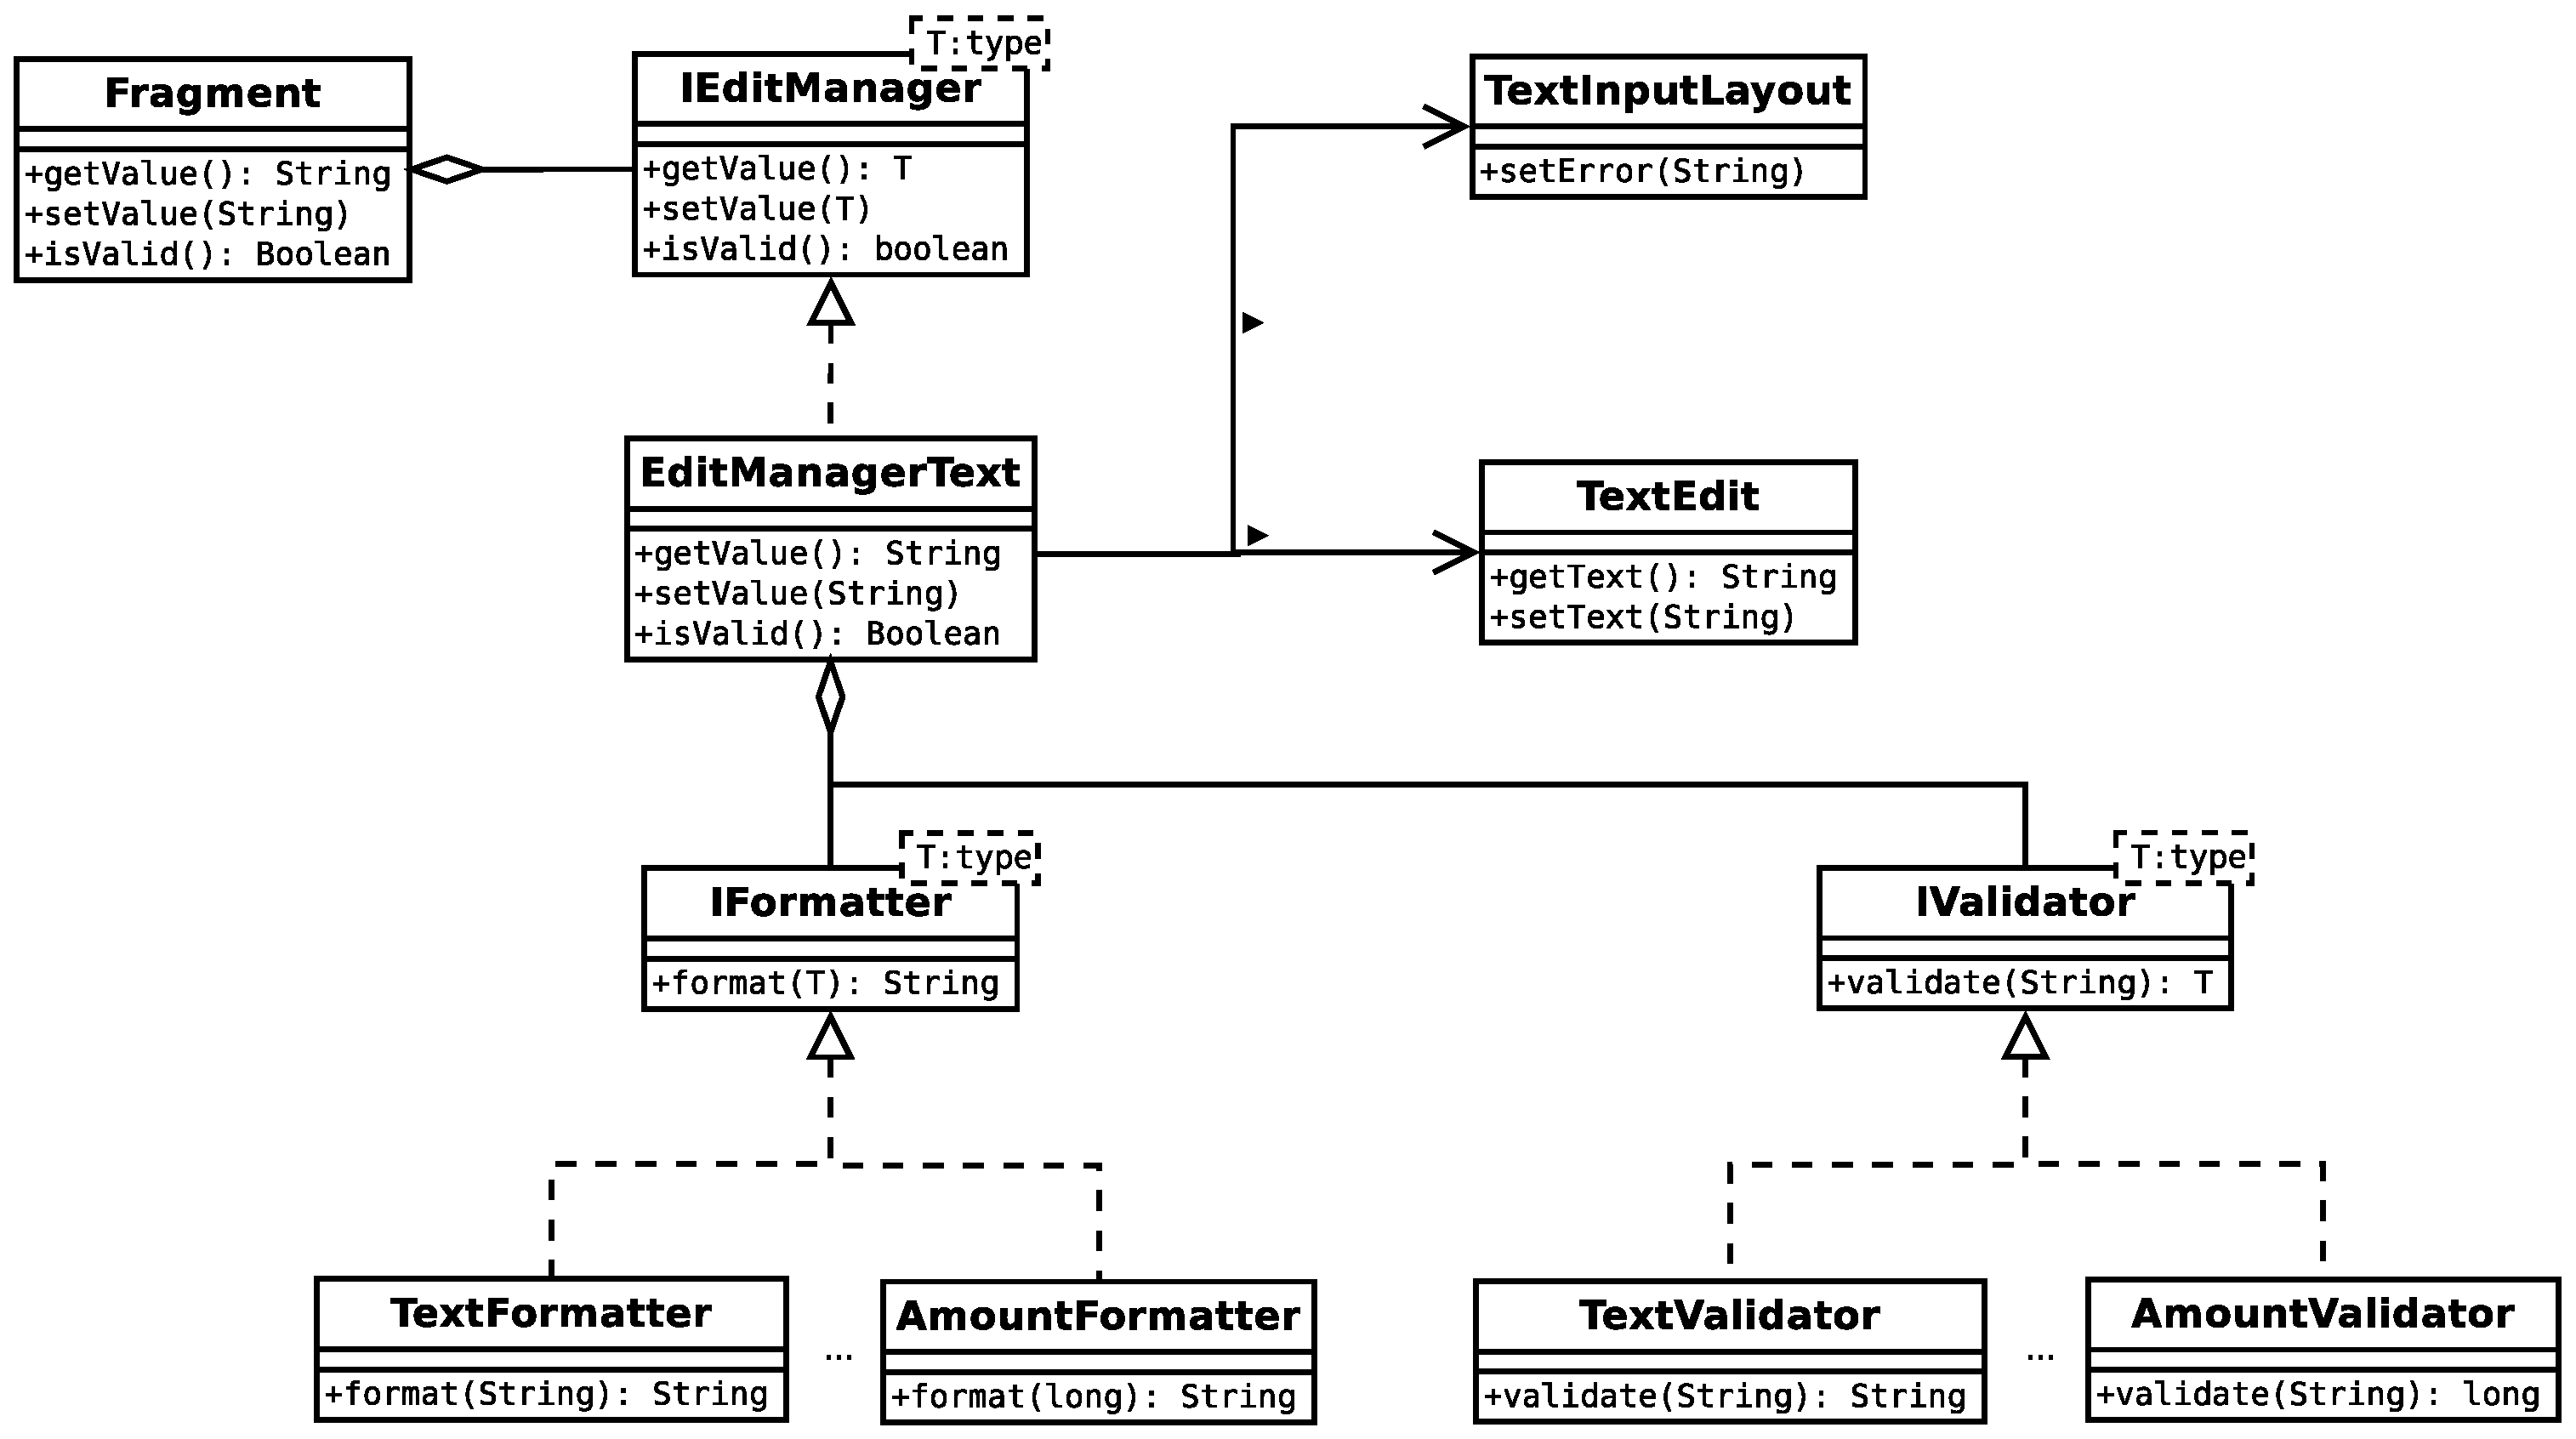
\includegraphics[width=140mm]{fig/implementation_ui_edit_manager.eps}
  }
  \caption{Диаграмма классов обработки данных, вводимых пользователем}
  \label{fig:implementation_ui_edit_manager}
\end{figure}

В нем определяются интерфейсы параметризованные интерфейсы
\texttt{IEditManager}, \texttt{IFormatter}, \texttt{IFormatter}
и набор их реализаций, связанных друг с другом. Рассмотрим каждый из них более подробно.

Интерфейс \texttt{IFormatter} используется для форматирования некоторого входного
значения заданного типа, определенного шаблоном интерфейса.
Результатом работы его единственного метода данного интерфейса является строка,
пригодная для размещения в элементе пользовательского интерфейса.

Метод \texttt{validate} интерфейса \texttt{IValidator} предназначен для
конвертации строки-параметра, сответствующей пользовательскому вводу,
в тип данных, совместимый с подсистемой обработки данных. В случае,
если подобная конвертация оказывается невозможной, он возбуждает
стандартное исключение типа \texttt{IllegalArgumentException}.

Интерфейс \texttt{IEditManager} определяет протокол взаимодействия
между фрагментом приложения, полем ввода данных
и подсистемой обработки данных.
Он имеет три метода, первые два из которых используются
для установки и получения последнего корректного введенного значения
в совместимом формате соответственно, а третий используется для проверки,
содержит ли поле ввода корректное значение в данный момент.

Взаимодействие описанных сущностей осуществляется следующим образом.
Экран или фрагмент в ходе своего жизненного цикла создают экземпляр класса,
реализующего интерфейс \texttt{IEditManager} и связывают его с целевыми
полями ввода и прочими вспомогательными объектами.
Конкретная реализация интерфейса \texttt{IEditManager}
(например, \texttt{EditManagerText})
создает необходимые ей экземлпяры классов, реализующих интерфейсы
\texttt{IFormatter} (\texttt{TextFormatter})
и \texttt{IValidator} (\texttt{TextValidator}),
и использует их в своей реализации,
подставляя результаты вызова методов объекто этих классов
в качестве собственных выходных значений.

Рассмотрим пользовательский интерфейс основных экранов приложения.
На рисунке~\ref{fig:implementation_ui_activity_balance_text}
представлен главный экран приложения в
текстовом режиме представления данных.

\begin{figure}[h!]
  \centering
  \fcolorbox{gray}{white}{
    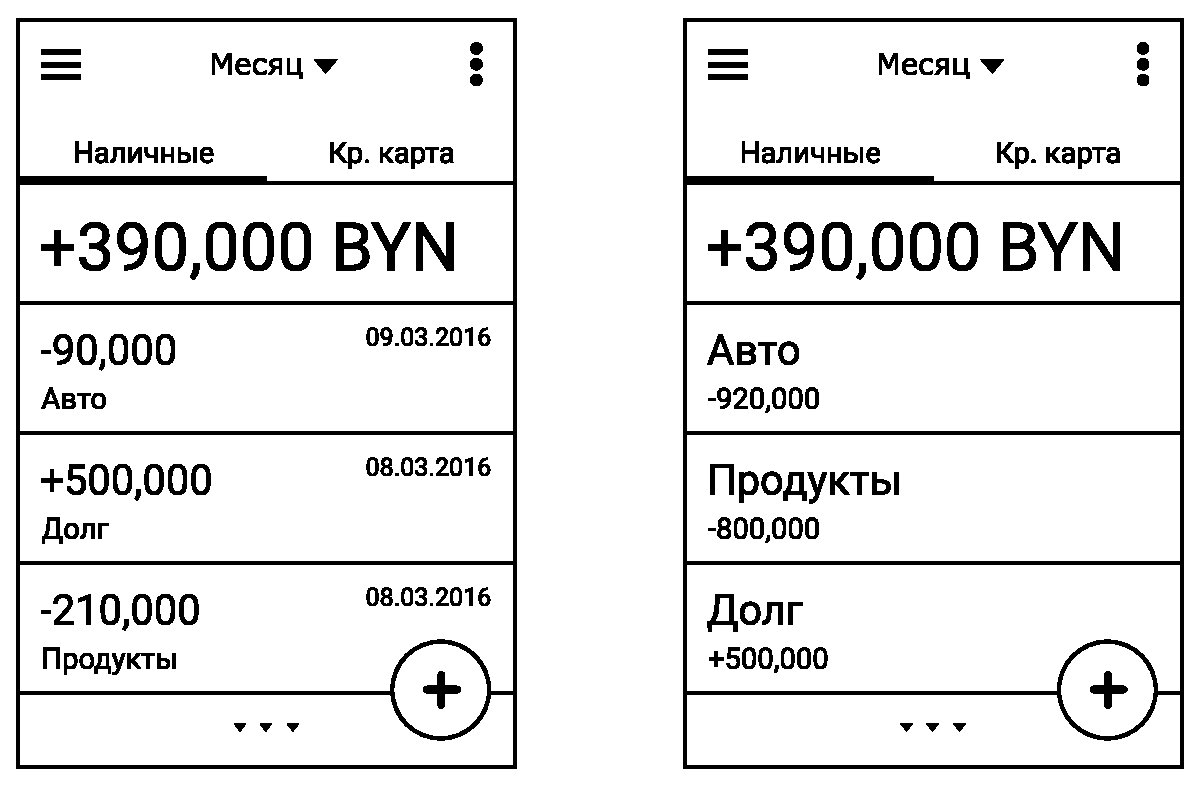
\includegraphics[width=140mm]{fig/implementation_ui_activity_balance_text.eps}
  }
  \caption{Главный экран (текстовый режим)}
  \label{fig:implementation_ui_activity_balance_text}
\end{figure}

Данный экран предназначен для отображения текущей финансовой
информации пользователя. Основными его элементами являются:
\begin{itemize}
\item виджет выбора промежутка учета;
\item виджет выбора учетной записи;
\item поле суммы денежных средств текущей учетной записи;
\item список связанных изменений баланса;
\item кнопка добавления изменения баланса.
\end{itemize}

По умолчанию элементы списка содержат величину изменения баланса,
список связанных категорий, а также дату регистрации изменения.
С помощью переключателя, расположенного во вспомогательном меню,
пользователь может включить группировку данных.
В этом случае список изменений баланса содержит сведения
об изменениях баланса за выбранный период,
сгрупированные по категориям учета.
При нажатии на любой элемент списка,
а также на кнопку добавления изменения баланса пользователь переходит
на экран редактирования изменения баланса,
при этом в случае редактирования существующей записи поля данного
экрана заполняются автоматически.
С помощью кнопок, расположенных в верхней части экрана, пользователь
может открыть главное меню приложения или вспомогательное меню экрана.
С помощью переключателя, расположенного во вспомогательном меню,
пользователь может перейти в графический режим, представленный
на рисунке~\ref{fig:implementation_ui_activity_balance_graphic}.

\begin{figure}[h!]
  \centering
  \fcolorbox{gray}{white}{
    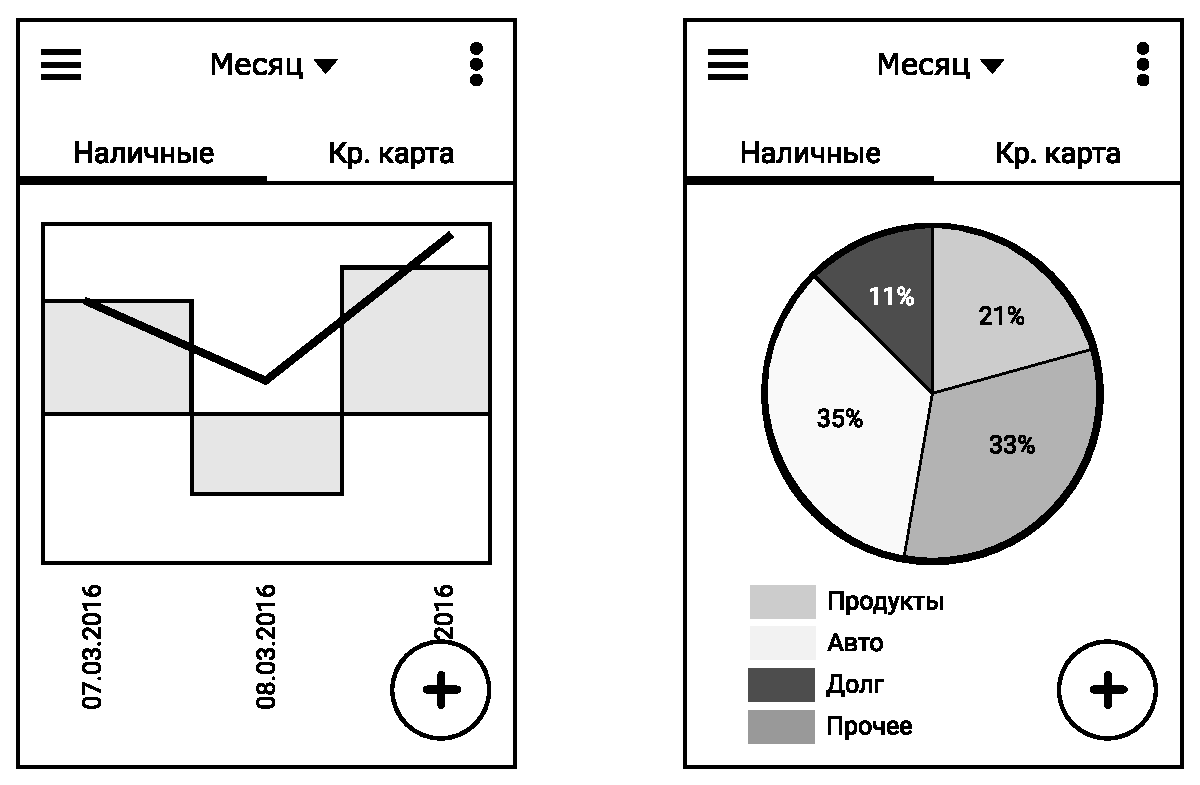
\includegraphics[width=140mm]{fig/implementation_ui_activity_balance_graphic.eps}
  }
  \caption{Главный экран (графический режим)}
  \label{fig:implementation_ui_activity_balance_graphic}
\end{figure}

Поведение данного экрана в графическом режиме также зависит от того,
включена ли группировка данных. Если она выключена,
пользователю показывается график изменения баланса выбранной
учетной записи за выбранный период.
На оси ординат данного графика расположены значения,
соответствующие величинам изменений баланса,
а на оси абсцисс --- даты учета.
График показывает как абсолютные значения изменений баланса,
сгруппированные по датам учета (в виде столбцов),
так и изменения интегрального показателя учета (в виде ломаной).
При включенной группировке данных пользователю показывается
круговая диаграмма, представляющая распределение изменений баланса
по категориям учета.

На рисунке~\ref{fig:implementation_ui_activity_input}
представлен экран редактирования изменений баланса.
Данный экран содержит переключатель типа изменения баланса (приход/расход),
поля ввода величины изменения баланса и даты учета, а также список
категорий учета, которые можно связать с данным изменением.
Поле даты учета имеет значение по умолчанию, соответствующее текущей дате.
С помощью кнопок, расположенных в верхней части экрана, пользователь
может сохранить изменения или вернуться на предыдущий экран.

\begin{figure}[h!]
  \centering
  \fcolorbox{gray}{white}{
    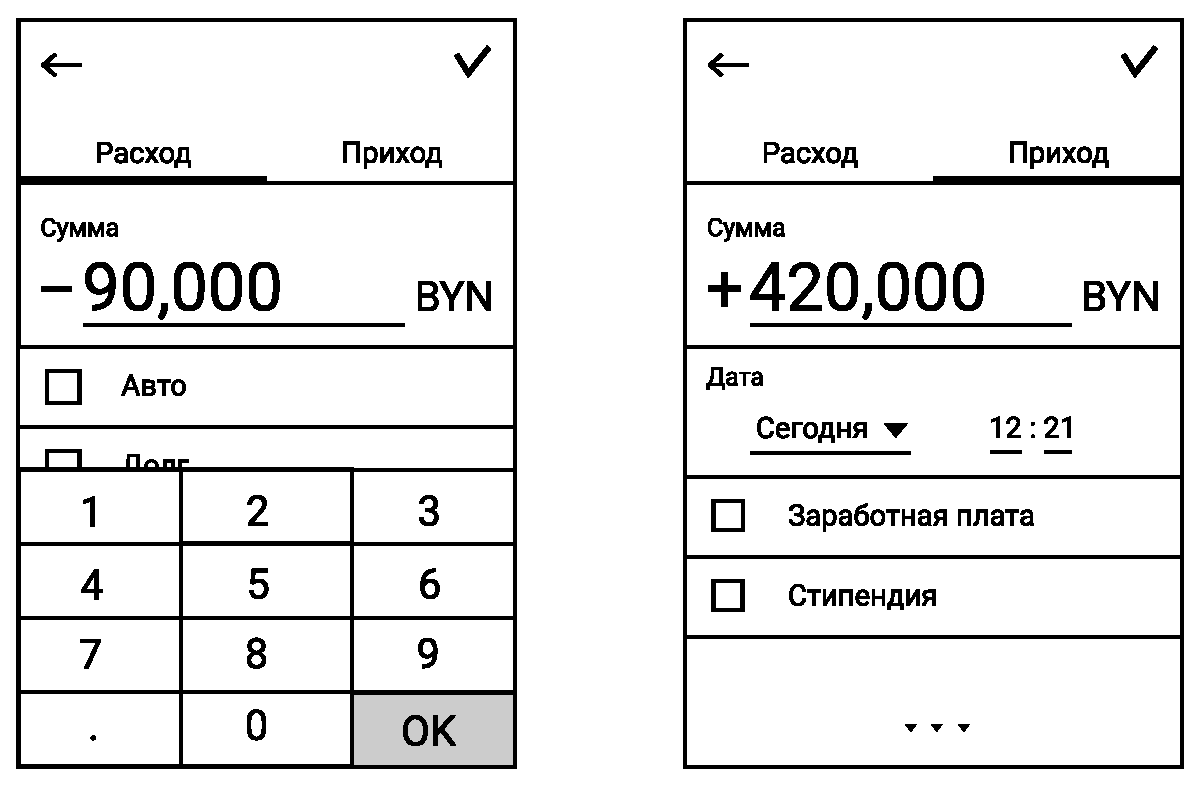
\includegraphics[width=140mm]{fig/implementation_ui_activity_input.eps}
  }
  \caption{Экран редактирования изменений баланса}
  \label{fig:implementation_ui_activity_input}
\end{figure}

На рисунке~\ref{fig:implementation_ui_activity_account}
представлены экраны просмотра и редактирования учетных записей.
Экран просмотра позволяет выполнять основные операции
со списком учетных записей.
Создание новых записей производится путем нажатия на кнопку,
расположенную в верхнем правом углу экрана просмотра списка записей.
Удаление записи производится путем сдвига соответствующего элемента списка;
редактирование --- путем нажатия на него.
Создание и редактирование учетных записей производится с помощью
отдельного экрана.
Кроме этого, пользователь имеет возможность выбора порядка следования
учетных записей. Для изменения порядка записи в списке требуется
выполнить долгое нажатие на данную запись и перетащить ее в требуемое место.

Экран редактирования позволяет добавить новую или изменить выбранную
учетную запись. Данный экран состоит из поля ввода названия учетной записи,
а также списка валют учета, из которого пользователю требуется выбрать необходимую.
С помощью кнопок, расположенных в верхней части экрана, пользователь
может сохранить изменения или вернуться на предыдущий экран.

\begin{figure}[h!]
  \centering
  \fcolorbox{gray}{white}{
    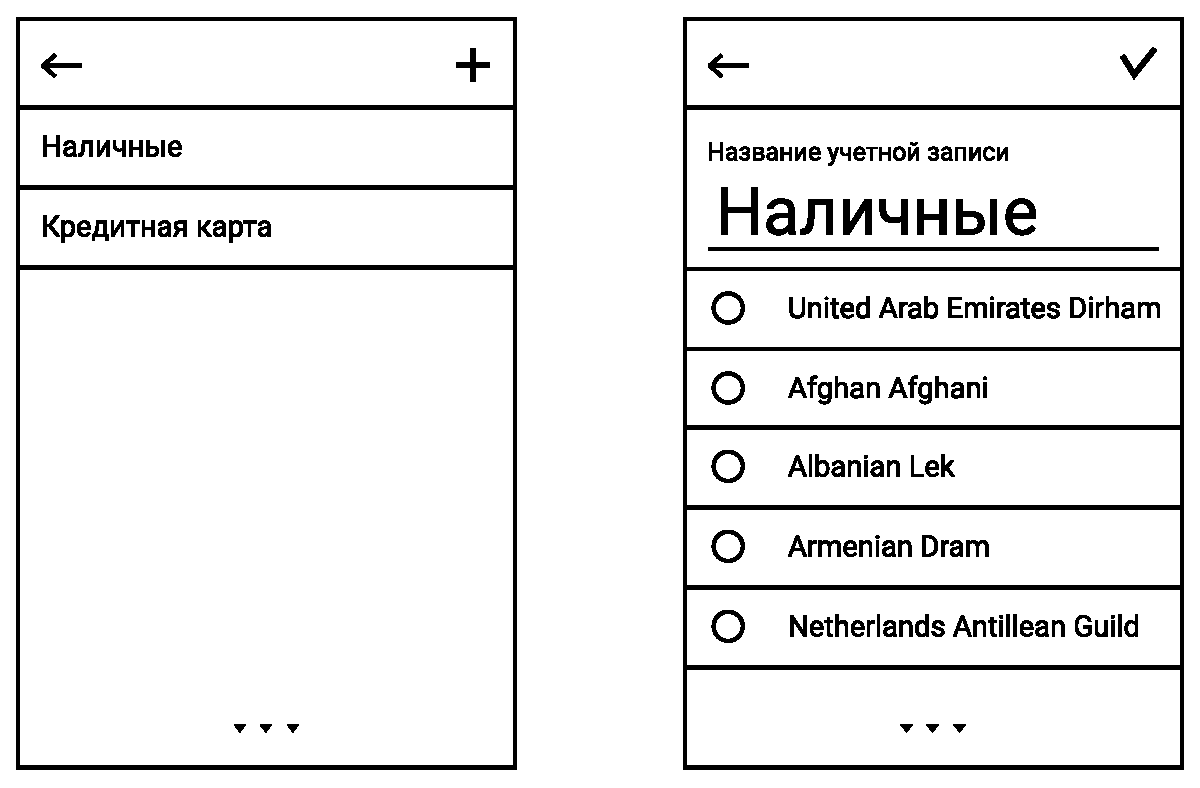
\includegraphics[width=140mm]{fig/implementation_ui_activity_account.eps}
  }
  \caption{Экраны управления учетными записями}
  \label{fig:implementation_ui_activity_account}
\end{figure}

На рисунке~\ref{fig:implementation_ui_activity_category}
представлены экраны просмотра и редактирования категорий учета.
Экран просмотра позволяет выполнять основные операции
со списком категорий ввода.
Создание новых категорий производится путем нажатия на кнопку,
расположенную в верхнем правом углу экрана просмотра списка записей.
Удаление записи производится путем сдвига соответствующего элемента списка;
редактирование --- путем нажатия на него.
Создание и редактирование категорий учета производится также
с помощью отдельного экрана.

Экран редактирования позволяет добавить новую или изменить выбранную
учетную запись. Данный экран состоит из поля ввода названия категории учета,
а также переключателя выбора типа категории (приход/расход).
С помощью кнопок, расположенных в верхней части экрана, пользователь
может сохранить изменения или вернуться на предыдущий экран.

\begin{figure}[h!]
  \centering
  \fcolorbox{gray}{white}{
    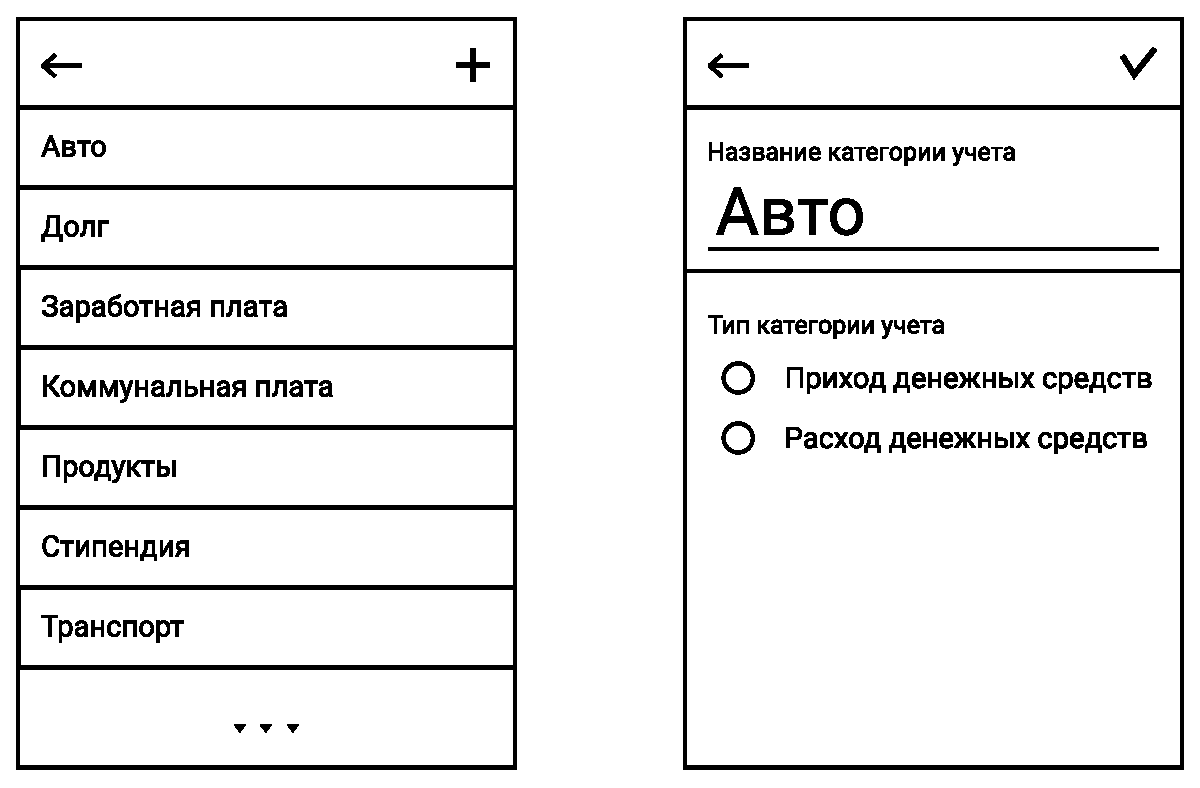
\includegraphics[width=140mm]{fig/implementation_ui_activity_category.eps}
  }
  \caption{Экраны управления категориями учета}
  \label{fig:implementation_ui_activity_category}
\end{figure}

Приложение имеет и некоторые другие экраны, например,
экран настроек или экран распознавания изображений.
Содержание и внешний вид данных экранов является объектом для
изменений, поэтому в данном разделе не рассматривается.
Схемы всех экранов представлены на плакатах графического материала.


\subsection{Реализация подсистемы обработки данных}
\label{subsec:implementation_bl}

Подсистема обработки данных представляет собой связующее звено
между подсистемами хранения данных, компьютерного зрения и
пользовательским интерфейсом и играет ключевую роль в работе всего приложения.
Поскольку данная подсистема соответствует блоку Presenter паттерна
MVP, ее реализация состоит из набора классов и интерфейсов,
имеющих в составе своего названия данное ключевое слово.

На рисунке~\ref{fig:implementation_bl_presenter} представлена схема взаимодействия
классов графического интерфейса и классов подсистемы обработки данных.
Классы \texttt{Activity} и \texttt{Fragment} в ходе своего жизненного цикла
создают объекты классов \texttt{PresenterActivity} и \texttt{PresenterFragment}.
Интерфейсы классов \texttt{Presenter*} имеют следующие особенности:
\begin{itemize}
  \item привязаны к жизненному циклу родительских объектов;
  \item принимают в качестве аргументов объекты типа \texttt{Bundle};
  \item инкапсулируют набор рабочих данных и объекты Realm.
\end{itemize}

Данные объекты также инкапсулируют все необходимые алгоритмы обработки данных и
имеют доступ к подсистеме хранения данных приложения (класс \texttt{DBManager}).
Объекты классов графического интерфейса перенаправляют
им свои запросы загрузки, обработки и хранения данных,
используя индексы требуемых им объектов в списках хранения данных.

\begin{figure}[h!]
  \centering
  \fcolorbox{gray}{white}{
    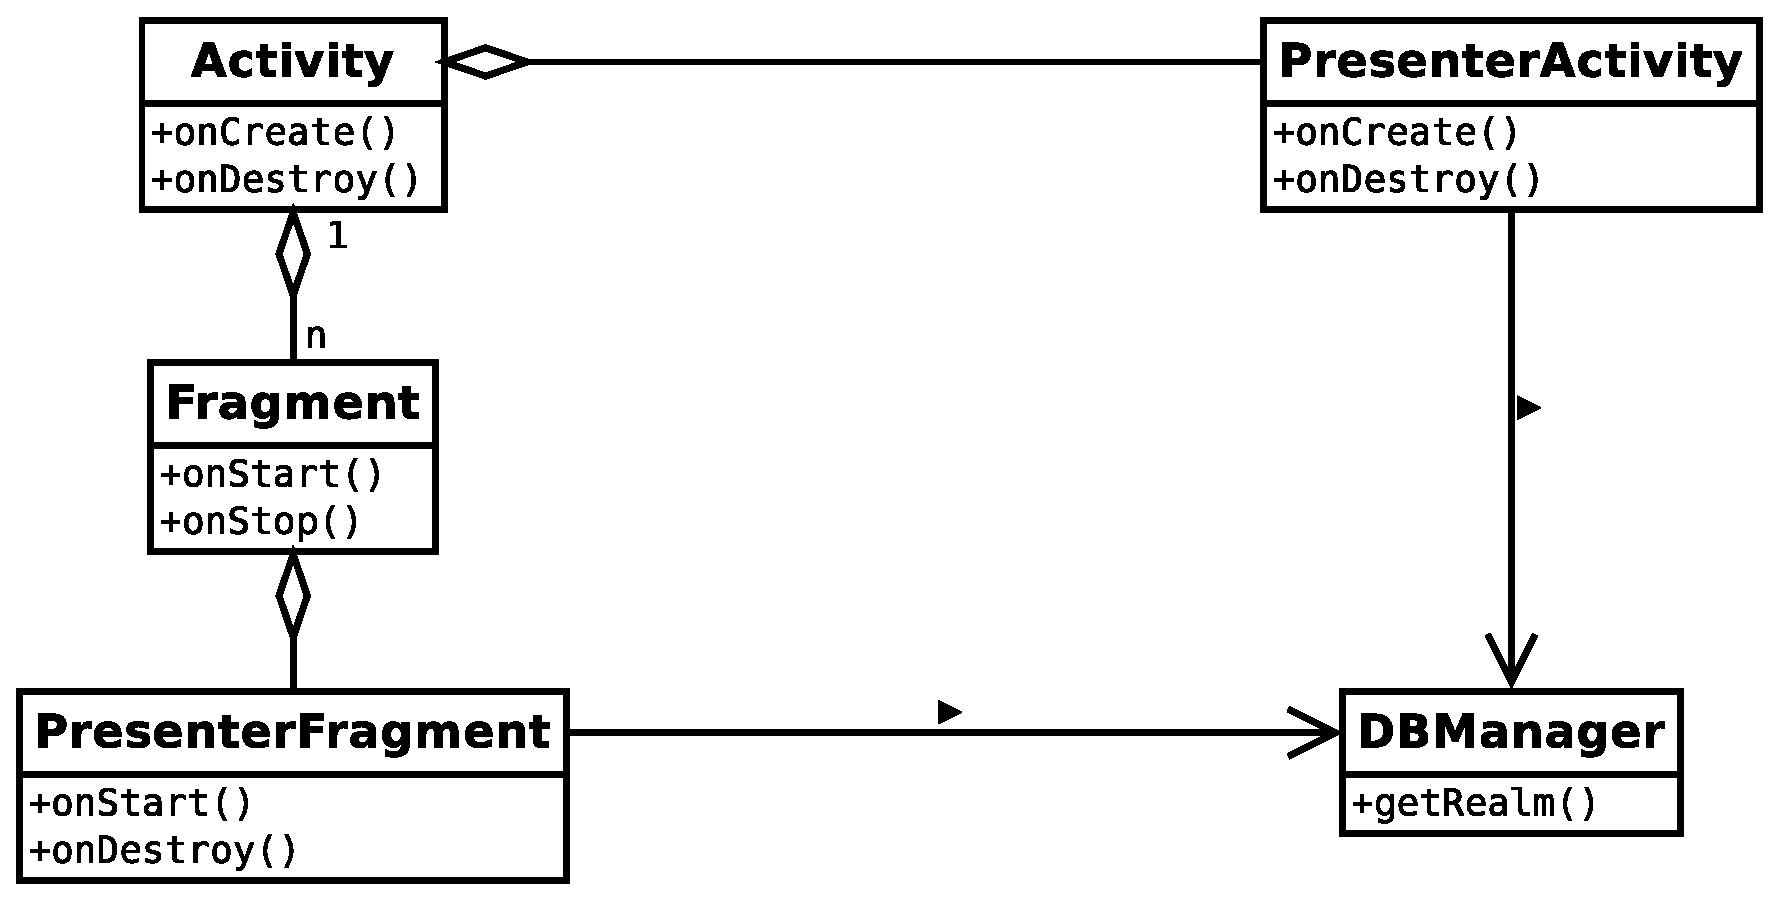
\includegraphics[width=140mm]{fig/implementation_bl_presenter.eps}
  }
  \caption{Схема использования классов \\ подсистемы обработки данных}
  \label{fig:implementation_bl_presenter}
\end{figure}

Подводя итог рассмотрению реализации частей приложения, отметим,
что в целом их структура разработана таким образом,
чтобы избегать циклов в графе взаимодействия их объектов.
Данная особенность позволила существенно упростить
структуру проекта в целом и его подсистем в частности.


% Реализация алгоритма распознавания изображений (OpenCV).

\subsection{Тестирование программного модуля}

Существует как минимум три основных метода тестирования
программного обеспечения:
\begin{itemize}
\item ручное;
\item автоматизированное;
\item юнит-тестирование.
\end{itemize}

Ручное тестирование представляет собой активное использование приложения
с целью выявления ошибок в его работе.
Автоматизированное тестирование отличается от ручного тем,
что в его случае сам алгоритм использования приложения также запрограммирован.
Данный вид тестирования, называемый также регрессионным,
позволяет сравнительно быстро определить,
внесли ли новые изменения в код приложения новые ошибки в ход его работы.
Юнит-тестирование используется по сути с той же целью,
что и автоматизированное. Основные отличия заключаются в том,
что юнит-тесты пишутся разработчиками приложения,
тестируют части кода приложения, а не все приложение в целом
и имеют значительно меньшие размер и время выполнения.

Существует некоторая специфика в механизме тестирования приложений
для платформы Android. Суть её сводится к разделению понятия юнит-тестов
на тесты, выполняемые на компьютере разработчика, и на инструментальные тесты,
выполняемые на целевом устройстве.
Основной причиной данного разделения является необходимость тестирования
графического интерфейса приложения и существование ошибок,
присущих конкретным версиям платформы.
С другой стороны, многие юнит-тесты принципиально не зависят от
целевой платформы и могут выполняться значительно быстрее
на компьютере разработчика
(это является возможным благодаря кроссплатформенности Java VM).

В рамках реализации данного проекта были разработан набор юнит-тестов,
покрывающих ключевую функциональность приложения.
Использование паттерна MVP позволило существенно их написание.
Дело в том, что одной из особенностей данного паттерна является возможность
определения интерфейсов \texttt{IPresenter*} и использования
их в классах-клиентах вместо конкретных реализаций \texttt{Presenter*},
как показано на рисунке~\ref{fig:implementation_testing_presenter}.

\begin{figure}[h!]
  \centering
  \fcolorbox{gray}{white}{
    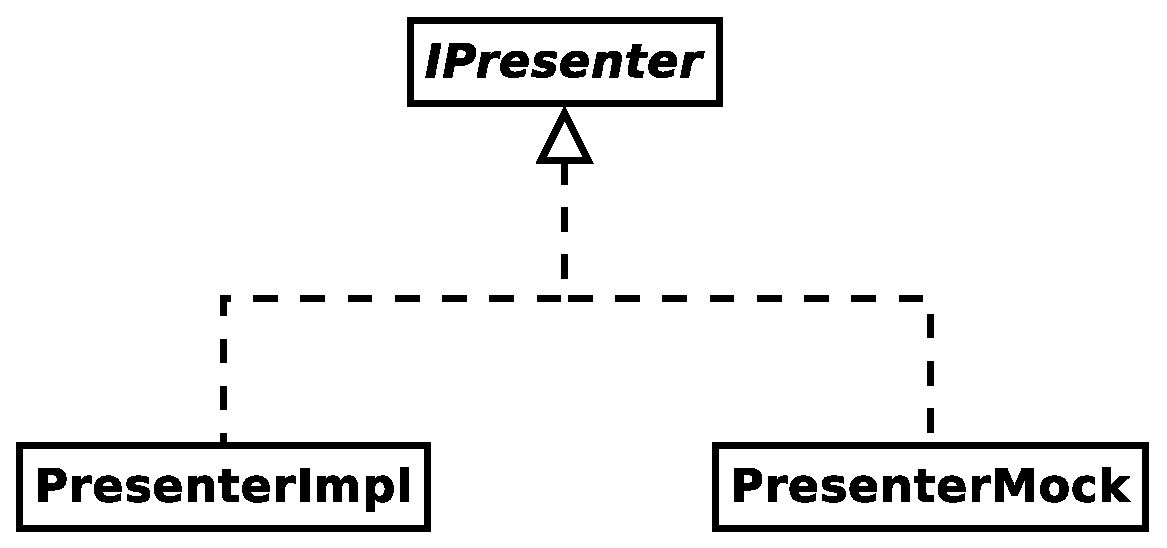
\includegraphics[width=140mm]{fig/implementation_testing_presenter.eps}
  }
  \caption{Схема использования классов \\ подсистемы обработки данных}
  \label{fig:implementation_testing_presenter}
\end{figure}

Данный подход преследует две цели:
\begin{itemize}
\item отделение интерфейса классов подсистемы обработки данных от реализации;
\item получение возможности использования классов-заглушек (\texttt{PresenterMock*}).
\end{itemize}

Классы-заглушки удобно использовать для тестирования классов подсистем-клиентов.
В начале теста производится создание объекта тестируемого класса,
сопровождающегося подменой используемого им \texttt{Presenter*}
на \texttt{PresenterMock*}.
Методы объектов классов-заглушек вместо действий, предписанных их контрактами,
выполняют действия, направленные на облегчение тестирования классов-клиентов:
логгирование, предоставление вымышленных данных,
эмулирование поведенения объектов <<настоящих>> классов.

\subsection{Руководство пользователя}

Установка приложения из Google Play.
Ввод данных. Просмотр данных. Группировка.
Скриншоты.

\subsection{Перспективы развития}

Сортировка категорий на основании данных геолокации.
% Распознавание суммы по чеку.